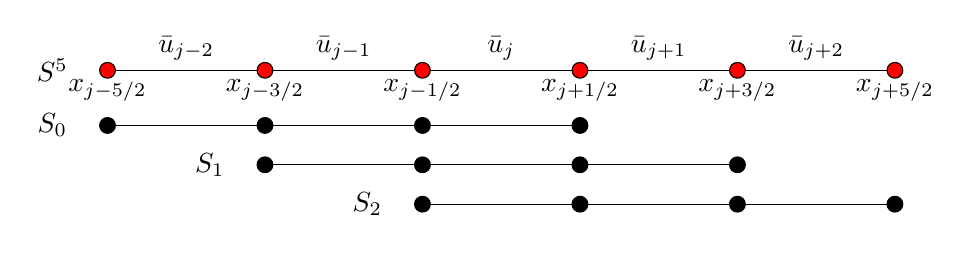
\begin{tikzpicture}
    \node[above] at (1,0) { $\bar{u}_{j-2}$ };
    \node[above] at (3,0) { $\bar{u}_{j-1}$ };
    \node[above] at (5,0) { $\bar{u}_{j}$ };
    \node[above] at (7,0) { $\bar{u}_{j+1}$ };
    \node[above] at (9,0) { $\bar{u}_{j+2}$ };

    \draw (0,0) -- (10,0);
    \foreach \x/\label in {0/{$x_{j-{5/2}}$},2/{$x_{j-{3/2}}$},4/{$x_{j-1/2}$},6/{$x_{j+1/2}$},8/{$x_{j+3/2}$},10/{$x_{j+5/2}$}} {
    \draw[fill=red] (\x,0) circle (0.1) node[below] {\label};
    }
    \node at (-0.7,0) { $S^5$ };

    \draw (0,-0.5-0.2) -- (6,-0.5-0.2);
    \foreach \x in {0,2,4,6} {
            \draw[fill=black] (\x,-0.5-0.2) circle (0.1) ;
        }
    \node at (-0.7,-0.5-0.2) { $S_0$ };

    \draw (2,-1-0.2) -- (8,-1-0.2);
    \foreach \x in {2,4,6,8} {
            \draw[fill=black] (\x,-1-0.2) circle (0.1) ;
        }
    \node at (1.3,-1-0.2) { $S_1$ };

    \draw (4,-1.5-0.2) -- (10,-1.5-0.2);
    \foreach \x in {4,6,8,10} {
            \draw[fill=black] (\x,-1.5-0.2) circle (0.1) ;
        }
    \node at (3.3,-1.5-0.2) { $S_2$ };

\end{tikzpicture}